\chapter{Anwendung: Oberflächenkrümmung}
  
  \begin{ziel}
    In vielen wissenschaftlichen Problemen kann die Krümmung
    einer Oberfläche eine entscheidene Rolle spielen. 
    Sie kann zum Beispiel ein wichtiger Bestandteil von Differentialgleichungen sein.
    So kommt die mittlere Krümmung \( H \) bei fluidmechanischen Formulierungen auf bewegliche Membranen 
    \( M_{t} \) in der
    Kontinuitätsgleichung
    \begin{align}
      \dot{\rho} + \rho\div\vec{v} - \rho v_{\vec{\nu}} H &= 0
    \end{align}
    vor (siehe \cite{desimone}).
    Ein weiteres einfaches Beispiel ist die Evolution von Oberflächen \( M_{t} \) über den mittleren
    Krümmungsfluss
    \begin{align}
      \dot{\vec{x}} = 2 H \vec{\nu} 
    \end{align}
    oder die Bestimmung des topologisch invarianten Geschlechts
    \begin{align}
      \mathfrak{g} = 1 - \frac{1}{4\pi}\int_{M}KdA
    \end{align}
    einer orientierten Mannigfaltigkeit \( M \) ohne Rand mit Gaußscher Krümmung \( K \),
    was dierekt aus dem Satz von Gauß-Bonnet 
    und den Zusammenhang für die Euler-Charakeristik \( \chi = 2-2\mathfrak{g} \) folgt.
    Unter den gewählten Voraussetzungen gibt \( \mathfrak{g} \) die Anzahl der "`Löcher"'/"`Poren"'/"`Henkel"' an.
    
    Es ließen sich noch weitere Beispiele finden in dem diverse Krümmungsgrößen für die Behandlung von
    Nöten wären.
    Oftmals liegt die Oberfläche allerdings nur als diskrete Eingangsgröße vor. 
    Somit sind viele
    geometrische Werte nicht bekannt und müssen Approximiert werden.
    Wir werden uns in diesem Kapitel speziell die Gaußsche und die mittlere Krümmung betrachten.
    Diese werden wir mit hilfe des DECs approximieren und zum einen mit den Ergebnissen von C.-J. Heine 
    \cite{heine} vergleichen und zum anderen, im Falle der Gauß-Krümmung, mit einer naiven 
    Gauß-Bonnet-Diskretisierung.
  \end{ziel}

\section{Weingartenabbildung}
\label{secWeingartenabbildung}
  Die Weingartenabbildung \( S \), auch Formoperator (Shapeoperator), ist im Prinzip die 2. Fundamentalform \( \II \) unter Beachtung der Metrik \(
 g \) (1. Fundamentalform).
  \( S \) gibt uns Informationen über die Gestalt von \( M \). 
  Sie misst in einer gewissen Weise wie sehr sich die Oberfläche von einer Ebenene unterscheidet, speziell ist \( M \) eine flache Ebene
  genau dann wenn die Weingartenabbildung identisch Null ist.
  Des Weiteren lassen sich aus der Weingartenabbildung die Hauptkrümmungen \( k_{1} \) und \( k_{2} \) herleiten und damit auch die
  Gaußkrümmung \( K = k_{1}*k_{2} \) und die mittlere Krümmung \( H = \frac{1}{2}\left( k_{1} + k_{2} \right) \).
  Die 1. Fundamentalform ist eine Größe der inneren Geometry und kann somit alleine auf der Oberfläche selbst bestimmt werden
  invariant gegenüber jeglicher Einbettungen/Parametrisierungen.
  Das ist bei der Weingartenabbildung anders, sie hängt von der äußeren Geometrie ab, d.h. die der Einbettung in einem Ambienteraum.
  In unserem Fall ist das der \( \R^{3} \) und die Weingartenabbildung lässt sich über das Normalenvektorfeld (Gaussabbildung)
  \begin{align}
    \vec{\nu} = \left[ \nu^{1}, \nu^{2}, \nu^{3} \right]^{T}: M &\rightarrow TN \subset \R^{3} \\
                         \vec{x} &\mapsto \vec{\nu}_{\vec{x}} \in T_{\vec{x}}N \bot T_{\vec{x}}M
  \end{align}
  berechnen. 
  Hierbei ist \( \vec{\nu}_{\vec{x}} \) der Normalenvektor im Punkt \( \vec{x} \) und \( T_{\vec{x}}N \) der eindimensionale Normalenraum
  der orthogonal zum Tangentialraum ist. 
  Da meistens klar ist, dass wir Punktweise arbeiten, kann auch hier die Indizierung weggelassen werden und wir schreiben nur 
  \( \vec{\nu} \) statt \( \vec{\nu}_{\vec{x}} \).
  \begin{definition}
    Die Weingartenabbildung ist in jedem Punkt der Oberfläche eine lineare Abbildung und definiert sich dort durch
    \begin{align}
      S: T_{\vec{x}}M &\rightarrow T_{\vec{x}}M \\
                    \vec{v} &\mapsto \exd\vec{\nu} \left( \vec{v} \right) \formkomma
    \end{align}
    wobei \( \exd\vec{\nu} \left( \vec{v} \right) \) der \( \R^{3} \)-Vektor der Richtungsableitungen in Richtung \( \vec{v}
    \) ist, wie sich einfach nachrechnen ließe (\( \vec{\nu} \) ist eine \( \R^{3} \)-vektorisierte 0-Form).
  \end{definition}
  Bei der Definition von \( S \) ist etwas Obacht geboten, weil sie oft auch mit negativen Vorzeichen definiert wird.
  Da wir uns aber vordergründig für dessen Eigenwerte interessieren spielt das Vorzeichen aber keine Rolle für uns.
  Anders als in \cite{heine} angegeben ist die Weingartenabbildung (\( (1,1) \)-Tensor) nicht die 2. Fundamentalform
  (\( (0,2) \)-Tensor). In der Matrixdarstellung unterscheiden sich beide in der Höhe der Indizes, das heißt
  \( S = \left(h^{i}_{\phantom{i}j}\right)\) und \( \II = \left( h_{ij} \right) \) oder anders geschrieben   \( S = (g)^{-1} \II \)
  (vgl. \cite{FirstCourse}).
  Somit sind auch die Eigenwerte beider Matrizen im Allgemeinen nicht gleich.
  Die Komponenten der Weingartenabbildung lassen sich für eine lokales orthogonales Koordinatensystem \( \left( x^{1},x^{2} \right) \)
  mit Riemannmetrik \( g=\diag{g_{1},g_{2}} \) berechnen durch
  \begin{align}
    h^{i}_{\phantom{i}j} &=  g^{i}h_{ij} = g^{i} \exd\vec{\nu}\left(\frac{\partial}{\partial x^{i}}\right) 
                                                  \cdot \frac{\partial}{\partial x^{j}} \\
                          &= \nabla_{i} \vec{\nu} \cdot \frac{\partial}{\partial x^{j}}
  \end{align}
  für \( i,j\in\left\{ 1,2 \right\} \) und \( \nabla_{i} \vec{\nu} \), die \( i \)-ten Komponente (Zeile) des Gradiente des
  Normalenvektors,
  das heißt
  \begin{align}
    \nabla\vec{\nu} &= \left( \exd \vec{\nu}\right)^{\sharp}
                     = \left( \sum_{k=1,2} \frac{\partial}{\partial x^{k}} \vec{\nu} dx^{k} \right)^{\sharp} \\
                    &= \sum_{k=1,2} g^{k}\frac{\partial}{\partial x^{k}} \vec{\nu}\frac{\partial}{\partial x^{k}}  \\
                    &=: \sum_{k=1,2} \nabla_{k}\vec{\nu}\frac{\partial}{\partial x^{k}} \formkomma
  \end{align}
  Zu beachten ist dabei, dass \( \nabla_{i} \) sich von der Richtungsableitung in der \( i \)-ten Basisrichtung um einen metrischen Faktor
  unterscheidet.

  Nun wollen wir aber nicht in lokalen sondern in globalen \( \R^{3} \)-Koordinaten rechnen in denen auch das Bild des Normalenvektorfeldes
  definiert ist. 
  Dazu definieren wir die erweiterte Weingartenabbildung in diesen Koordinaten.
  \begin{definition}
    Die erweiterte Weingartenabbildung \( \bar{S} \) sei an jedem Punkt der Oberfläche gegeben durch
    \begin{align}
      \bar{S}:= \nabla\vec{\nu} \in \R^{3 \times 3} \formpunkt
    \end{align}
    Dabei sei das Ableiten in Normalenrichtung zulässig ergibt jedoch den Wert Null (konstante Erweiterung in Normalenrichtung).
  \end{definition}
  Die erweiterte Weingartenabbildung eingeschränkt auf \( T_{\vec{x}}M \)\ in lokalen Koordinaten ist dann gerade \( S \),
  \todo{genauer}
  wobei die Eigenwerten von \( \bar{S} \) gleich \( \left\{ k_{1},k_{2},0 \right\} \) sind.
  Einen Beweis dazu findet sich in \cite{kimura} (Part 2, Kap. 2).
  
  \subsection{Implementierung}
    Die Komponenten der erweiterte Weingartenabbildung können wir nun mit Hilfe des diskreten Primär-Dual-Gradienten im Mittel approximieren, das heißt
    \begin{align}
      \bar{h}^{i}_{\phantom{i}j} &= \left[ \nabla\vec{\nu} \right]_{ij} = \nabla_{j}\nu^{i}
                                 \approx \left[ \nabla^{\overline{pd}}\nu^{i} \right]_{j}
                                 =: \left[ S^{\overline{pd}} \right]_{ij}
    \end{align}
    mit \( i,j \in \left\{ 1,2,3 \right\} \).
    Für die Berechnung der Eigenwerte \( \left\{ \lambda_{0}, \lambda_{1}, \lambda_{2} \right\} \) an jedem Gitterpunkt 
    nutzen wir den von der MTL4 (Matrix Template Library 4) bereitgestellten QR-Algorithmus.
    Der betragsmäßig kleinste Eigenwert, der annährend null ist, ist o.E.d.A. \( \lambda_{0} \).
    Somit können die Gaußsche Krümmung und die mittlere Krümmung durch
    \begin{align}
      K &\approx \lambda_{1}*\lambda_{2} \formtext{bzw.} \\
      H &\approx \frac{1}{2}\left( \lambda_{1}+\lambda_{2}\right)    
    \end{align}
    approximiert werden.
    Die Weingartenabbildung \( S \) ist symmetrisch, das können wir von der numerisch ermittelten nicht exakt erwarten.
    Deshalb berechnen wir auch alle Einträge von \( S^{\overline{pd}} \) und nicht nur die obere oder untere Dreicksmatrix. 
    Die Eigenwerte können dann über die symmetrisch gemittelten Matrix erhalten werden, also von der Matrix
    \begin{align}
      \frac{1}{2} \left( S^{\overline{pd}} + \left( S^{\overline{pd}} \right)^{T} \right) \formpunkt
    \end{align}
    Mit dem Normalenraum auf den Gitterpunkten haben wir das gleiche Problem, wie schon mit dem Tangentialraum.
    Es ist nicht klar wo der Normalenraum auf den Ecken des Polyeders \( |K| \) liegen soll, denn eindeutig ist er nur auf den Inneren der Dreiecke
    bzw. auf den Voronoiecken.
    Deshalb mitteln wir wieder über einen 1-Ring des Primärgitterpunktes \( v \) zu
    \begin{align}
    \label{eqNormalMittel}
    \begin{aligned}
      \vecover{\nu}{\av}(v) &= \left\langle \vecover{\nu}{\av}, v \right\rangle 
          := \frac{1}{\left| \star v \right|} \sum_{\sigma^{2}\succ v} \left| \star v \cap \sigma^{2}\right| 
                      \left\langle \vec{\nu}, \star\sigma^{2} \right\rangle \\
          &= \frac{1}{\left| \star v \right|} \sum_{\sigma^{2}\succ v} \left| \star v \cap \sigma^{2}\right| 
                                          \vecover{\nu}{\sigma^{2}} \formpunkt
    \end{aligned}
    \end{align}
    Die Elementnormalen \( \vecover{\nu}{\sigma^{2}} \) werden von AMDiS bereit gestellt.
    Wenn wir \( \vec{\nu}_{i} \) wieder im "`Dualem"' lösen wollen, das heißt anwenden des HodgeOperators auf die Gleichung
    \eqref{eqNormalMittel} und damit durchmultiplizieren der Gleichung mit \( \left| \star v_{i} \right| \), dann können auch hier die
    Eckennormalen elementweise bestimmt werden.
    Dadurch ergibt sich das lineare Gleichungssystem
    \begin{align}
        \label{eqWeingartenEq1}
        \left\langle *\bar{\nu}^{i} , \star v \right\rangle 
                &= \left\langle *\left[ \vecover{\nu}{\av} \right]_{i}, \star v \right\rangle \\
        \label{eqWeingartenEq2}
        \left\langle *\left[ \nabla^{\overline{pd}}\bar{\nu}^{i} \right]_{j} , \star v \right\rangle
            - \left\langle *\left[ S^{\overline{pd}} \right]_{ij} , \star v \right\rangle 
                &= 0
    \end{align}
    für alle \( i,j\in\left\{ 1,2,3 \right\} \) und \( v\in K^{(0)} \) in dem alle Operatoren elementweise bestimmt werden können.
    Zusammen ergibt das 12 DOFs pro Knoten \( v \).
    Gleichung \eqref{eqWeingartenEq1} (3 Dofs pro Knoten) und \eqref{eqWeingartenEq2} (9 Dofs pro Knoten) 
    könnenten zwar auch seperat gelöst werden wodurch wir
    Speichervorteile hätten, aber das Lösen der beiden kleineren Gleichungssystem wäre nicht schneller, da der Lösungsaufwand für die
    resultierenden dünnbesetzten Systeme mit angepassteen Lösern etwa linear ist.
    Hinzu würden außerdem noch Initialisierungskosten kommen.

    Eine alternative Möglichkeit an die Normalen an einer Ecke \( v \) zu mitteln ist eine Mittelung über die Elementnormalen ohne
    Wichtung, das heißt
    \begin{align}
      \label{eqNormalConnMittel}
      \begin{aligned}
      \vecover{\nu}{\conn}(v) &= \left\langle \vecover{\nu}{\conn}, v \right\rangle 
          := \frac{1}{m_{v}} \sum_{\sigma^{2}\succ v}
                      \left\langle \vec{\nu}, \star\sigma^{2} \right\rangle \\
          &= \frac{1}{m_{v}} \sum_{\sigma^{2}\succ v}
                                          \vecover{\nu}{\sigma^{2}} \formkomma
     \end{aligned}
    \end{align}
    wobei \( m_{v} = \sum_{\sigma^{2}\succ v} 1 \in \mathds{N}_{+}\) die Anzahl der \( 2 \)-Simplizes im 1-Ring um \( v \) ist.
    Das Problem hierbei ist, dass \( m_{v} \) a priori auf einem einzelnen Dreieckselement nicht bekannt ist und damit vor dem Assemblieren
    der Systemmatrix zusätzliche globale Arbeit in die Bestimmung aller \( m_{v} \) gesteckt werden muss.
    
    \begin{beispiel}[Torus]
      Auf dem Torus sind die Gaußkrümmung \( K \), die mittlere Krümmung \( H \) und die Normalen \( \vec{\nu} \) bekannt (siehe Appendix
      \ref{torus}) und stehen uns zum vergleichen bzw. als Eingangsgröße zur Verfügung.
      Die Weingartenabbildung wurde als Gradient der exakten Normalen \( \vec{\nu} \) (Tab. \ref{tabWeingartenFehlerTorusExN})
      und der beiden hier vorgestellten gemittelten Normalen 
      \( \vecover{\nu}{\av} \) (Tab. \ref{tabWeingartenFehlerTorusAvN}) und 
      \( \vecover{\nu}{\conn} \) (Tab. \ref{tabWeingartenFehlerTorusConnN}) berechnet.
      Es werden wieder die relativen Fehler für die Auswertung benutzt.
      Für die Approximation der Krümmungsgrößen mit den exakten Normalen bekommen wir etwa eine experimentelle Konvergenzordnung von 2.
      Gerade in der Maximumsnorm überascht das ein wenig, da in Beispiel \ref{bspGradTorus} der diskrete Gradient auf feineren Gitter eine
      schlechteres Konvergenzverhalten aufwies.
      Bei den beiden Berechnungen mit den gemittelten Normalen bricht die Konvergenzrate bei feineren Gittern ein. 
      Wobei die Approximation der Weingartenabbildung mit \( \vecover{\nu}{\conn} \) noch etwas besser ausfällt als mit \(
      \vecover{\nu}{\av} \).
      In Abbildung \ref{figWeingartenFehlerTorus} ist zudem noch der Fehler von \( \vecover{\nu}{\av} \) aufgetragen 
      (der von \( \vecover{\nu}{\conn} \) ist ähnlich).
      Wie wir sehen liegt das schlechte Konvergenzverhalten nicht primär an die Mittelung der Normalen an sich.
      Vermutlich kommt es bei kleiner werdenen \( h \) zur starken Rundungsfehlern bei der Differenz in der Gradientenbildung, denn
      hier werden zwei Werte von einander abgezogen, die auf überlappenden Bereichen gemittelt werden. 
      In Abbildung \ref{figMeanTorus} ist die mittlere Krümmung und die lokalen absoluten Fehler für die Berechnung mit \(
      \vecover{\nu}{\av} \) abgebildet.
      Auch hier können wieder gewisse Strukturen im Fehlerbild erkannt werden, was darauf schließen lässt, dass der Fehler von der Gestalt
      der Dreieckselemente und seinen Nachbarn abhängt, denn auf den Niveaulinien des Fehlers sind die Gitter nahezu gleich.
      Hierbei konnte eine Verbindung zu diversen Gitterqualitätsmaßen
      \footnote{die von ParaView zur Verfügung stehen, z.B. \texttt{Radius Ratio}, \texttt{Aspect Frobenius}, \texttt{Maximum Angle}, usw.}
      nicht hergestellt werden.
      \begin{table}[htbp]
      \footnotesize
      \centering
      \begin{tabular}{|r|r|r|r|r|r|r|r|r|r|}
      \hline
      \multicolumn{1}{|c|}{DOFs} & \multicolumn{1}{c|}{\( h \)} & \multicolumn{1}{c|}{\( \err_{2}^{K} \)} & \multicolumn{1}{c|}{EOC} & 
        \multicolumn{1}{c|}{\( \err_{\max}^{K} \)} & \multicolumn{1}{c|}{EOC} & \multicolumn{1}{c|}{\( \err_{2}^{H} \)} &
        \multicolumn{1}{c|}{EOC} & \multicolumn{1}{c|}{\( \err_{\max}^{H} \)} & \multicolumn{1}{c|}{EOC} \\ \hline
        1360 & 0.263 & 4.21E-02 & \multicolumn{1}{l|}{} & 1.18E-01 & \multicolumn{1}{l|}{} & 1.59E-02 & \multicolumn{1}{l|}{} & 1.84E-02 & \multicolumn{1}{l|}{} \\ \hline
2016 & 0.215 & 2.77E-02 & 2.06 & 7.85E-02 & 2.02 & 1.11E-02 & 1.76 & 1.28E-02 & 1.79 \\ \hline
4752 & 0.138 & 1.16E-02 & 1.98 & 3.64E-02 & 1.75 & 4.97E-03 & 1.83 & 5.64E-03 & 1.86 \\ \hline
10192 & 0.094 & 5.42E-03 & 1.97 & 1.72E-02 & 1.93 & 2.38E-03 & 1.90 & 2.71E-03 & 1.89 \\ \hline
24640 & 0.060 & 2.26E-03 & 1.97 & 7.44E-03 & 1.89 & 1.01E-03 & 1.94 & 1.15E-03 & 1.93 \\ \hline
48832 & 0.043 & 1.15E-03 & 1.98 & 3.71E-03 & 2.03 & 5.14E-04 & 1.96 & 5.91E-04 & 1.95 \\ \hline
100480 & 0.030 & 5.61E-04 & 1.97 & 1.88E-03 & 1.88 & 2.52E-04 & 1.97 & 2.94E-04 & 1.93 \\ \hline
250992 & 0.019 & 2.26E-04 & 1.98 & 7.04E-04 & 2.14 & 1.01E-04 & 1.98 & 1.25E-04 & 1.87 \\ \hline
      \end{tabular}
      \caption[Gauß-/mittlere Krümmung aus Weingartenabb. auf Torus (ExN)]{Fehler von \( K \) und \( H \) (aus Weingartenabb. und
      exakten Normalen) (*ExN) auf dem Torus.}
      \label{tabWeingartenFehlerTorusExN}
      \vspace{10pt}
      \begin{tabular}{|r|r|r|r|r|r|r|r|r|r|}
      \hline
      \multicolumn{1}{|c|}{DOFs} & \multicolumn{1}{c|}{\( h \)} & \multicolumn{1}{c|}{\( \err_{2}^{K} \)} & \multicolumn{1}{c|}{EOC} & 
        \multicolumn{1}{c|}{\( \err_{\max}^{K} \)} & \multicolumn{1}{c|}{EOC} & \multicolumn{1}{c|}{\( \err_{2}^{H} \)} &
        \multicolumn{1}{c|}{EOC} & \multicolumn{1}{c|}{\( \err_{\max}^{H} \)} & \multicolumn{1}{c|}{EOC} \\ \hline
      1360 & 0.263 & 6.01E-02 & \multicolumn{1}{l|}{} & 1.20E-01 & \multicolumn{1}{l|}{} & 2.68E-02 & \multicolumn{1}{l|}{} & 3.77E-02 & \multicolumn{1}{l|}{} \\ \hline
      2016 & 0.215 & 4.06E-02 & 1.93 & 8.15E-02 & 1.90 & 1.87E-02 & 1.77 & 2.75E-02 & 1.55 \\ \hline
      4752 & 0.138 & 1.77E-02 & 1.89 & 3.86E-02 & 1.71 & 8.33E-03 & 1.84 & 1.23E-02 & 1.84 \\ \hline
      10192 & 0.094 & 8.65E-03 & 1.85 & 1.77E-02 & 2.02 & 4.07E-03 & 1.86 & 7.68E-03 & 1.21 \\ \hline
      24640 & 0.060 & 4.13E-03 & 1.67 & 1.44E-02 & 0.46 & 2.14E-03 & 1.44 & 8.90E-03 & -0.33 \\ \hline
      48832 & 0.043 & 2.79E-03 & 1.14 & 1.01E-02 & 1.03 & 2.02E-03 & 0.18 & 6.35E-03 & 0.98 \\ \hline
      100480 & 0.030 & 2.18E-03 & 0.68 & 9.68E-03 & 0.11 & 1.82E-03 & 0.29 & 6.08E-03 & 0.12 \\ \hline
      250992 & 0.019 & 1.61E-03 & 0.66 & 1.07E-02 & -0.22 & 1.29E-03 & 0.74 & 5.50E-03 & 0.22 \\ \hline
      \end{tabular}
      \caption[Gauß-/mittlere Krümmung aus Weingartenabb. auf Torus (AvN)]{Fehler von \( K \) und \( H \) (aus Weingartenabb. und
      gemittelten Normalen nach \eqref{eqNormalMittel}) (*AvN) auf dem Torus.}
      \label{tabWeingartenFehlerTorusAvN}
      \vspace{10pt}
      \begin{tabular}{|r|r|r|r|r|r|r|r|r|r|}
      \hline
      \multicolumn{1}{|c|}{DOFs} & \multicolumn{1}{c|}{\( h \)} & \multicolumn{1}{c|}{\( \err_{2}^{K} \)} & \multicolumn{1}{c|}{EOC} & 
        \multicolumn{1}{c|}{\( \err_{\max}^{K} \)} & \multicolumn{1}{c|}{EOC} & \multicolumn{1}{c|}{\( \err_{2}^{H} \)} &
        \multicolumn{1}{c|}{EOC} & \multicolumn{1}{c|}{\( \err_{\max}^{H} \)} & \multicolumn{1}{c|}{EOC} \\ \hline
        1360 & 0.263 & 5.90E-02 & \multicolumn{1}{l|}{} & 1.13E-01 & \multicolumn{1}{l|}{} & 2.48E-02 & \multicolumn{1}{l|}{} & 2.92E-02 & \multicolumn{1}{l|}{} \\ \hline
2016 & 0.215 & 4.02E-02 & 1.89 & 7.77E-02 & 1.84 & 1.73E-02 & 1.76 & 2.11E-02 & 1.59 \\ \hline
4752 & 0.138 & 1.75E-02 & 1.89 & 3.62E-02 & 1.74 & 7.75E-03 & 1.83 & 9.45E-03 & 1.83 \\ \hline
10192 & 0.094 & 8.39E-03 & 1.91 & 1.71E-02 & 1.95 & 3.75E-03 & 1.88 & 5.73E-03 & 1.30 \\ \hline
24640 & 0.060 & 3.64E-03 & 1.88 & 7.49E-03 & 1.85 & 1.78E-03 & 1.68 & 5.86E-03 & -0.05 \\ \hline
48832 & 0.043 & 2.12E-03 & 1.58 & 4.81E-03 & 1.29 & 1.41E-03 & 0.68 & 3.94E-03 & 1.15 \\ \hline
100480 & 0.030 & 1.39E-03 & 1.16 & 4.23E-03 & 0.36 & 1.19E-03 & 0.47 & 3.31E-03 & 0.48 \\ \hline
250992 & 0.019 & 8.84E-04 & 0.99 & 3.73E-03 & 0.27 & 8.24E-04 & 0.80 & 2.51E-03 & 0.60 \\ \hline
      \end{tabular}
      \caption[Gauß-/mittlere Krümmung aus Weingartenabb. auf Torus (ConnN)]{Fehler von \( K \) und \( H \) (aus Weingartenabb. und
      gemittelten Normalen nach \eqref{eqNormalConnMittel}) (*ConnN) auf dem Torus.}
      \label{tabWeingartenFehlerTorusConnN}
      \end{table}
       
      \begin{figure}
        \begin{minipage}[t]{0.49\textwidth}
          \centering\includegraphics[width=\textwidth]{bilder/Curvature/TorusKWein2Plot.eps}
        \end{minipage} \hfill
        \begin{minipage}[t]{0.49\textwidth}
          \centering\includegraphics[width=\textwidth]{bilder/Curvature/TorusKWeinMaxPlot.eps}
        \end{minipage}\\
        \begin{minipage}[t]{0.49\textwidth}
          \centering\includegraphics[width=\textwidth]{bilder/Curvature/TorusHWein2Plot.eps}
        \end{minipage}\hfill
        \begin{minipage}[t]{0.49\textwidth}
          \centering\includegraphics[width=\textwidth]{bilder/Curvature/TorusHWeinMaxPlot.eps}
        \end{minipage}
        \caption[Fehler Gauß-/mittlere Krümmung aus Weingartenabb. auf Torus]
                {(LogLogPlot) Fehler in diskreter \( L_{2} \)- und Maximumsnorm für die Gaußkrümmung \( K \) bzw. mittlere Krümmung \( H \) berechnet aus
                der Weingartenabbildung mit exakten Normalen (KExN)/(HExN), 
                nach \eqref{eqNormalMittel} gemittelte Elementnormalen (KAvN)/(HAvN) 
                und nach \eqref{eqNormalConnMittel} gemittelte Elementnormalen (KConnN)/(HConnN).
                Zudem ist auch der Fehler der Normalenmittelung nach \eqref{eqNormalMittel} in der jeweiligen Norm zusehen (AvN).}
        \label{figWeingartenFehlerTorus}
      \end{figure}
    \end{beispiel}

    \begin{fazit}
      Wenn die Normalvektoren an jedem Koten der Obeflächentriangulierung bekannt sind, zum Beispiel aus einer Parametrisierung
      \( \vec{x}: \left( u,v \right) \mapsto \left( x,y,z \right)\) durch
      \begin{align}
        \vec{\nu} &= \frac{\frac{\partial\vec{x}}{\partial u} \times \frac{\partial\vec{x}}{\partial v}}
                             {\left\| \frac{\partial\vec{x}}{\partial u} \times \frac{\partial\vec{x}}{\partial v} \right\|}
      \end{align}
      oder einer signierten Distanzfunktion \( \varphi \) durch
      \begin{align}
        \vec{\nu} &= \frac{\nabla_{\R^{3}}\varphi}{\left\| \nabla_{\R^{3}}\varphi \right\|} \formkomma
      \end{align}
      dann können mit der diskreten Weingartenabbildung gute Ergebnisse erziehlt werden.
      Sind dagegen die Normalen nicht bekannt, so muss in zunkünftigen Arbeiten entweder eine angepasstere Möglichkeit bereitgestellt
      werden die Normalen an den Ecken des Polyeders zu gewinnen oder ein für diese Problemstellung geeigneter diskreter Gradient,
      zum Beispiel ein Dual-Primär-Gradient für eine diskrete duale \( 0 \)-Form ausgewerten auf den primären Gitterpunkten.
      Hätten wir so einen Gradienten, dann könnten die Elementnormalen \( \vecover{\nu}{\sigma^{2}} \)direkt auswerten für eine
      Berechnung der diskreten Weingartenabbildung auf den Ecken.

      In Abschnitt \ref{secNumEx} wird zudem die hier vorgestellte Krümmungsapproximation auch auf anderen Oberflächen getestet und mit den
      Ergebnissen von \cite{heine} verglichen.
    \end{fazit}



\section{Krümmungsvektor}
  Der Krümmungsvektor \( \vec{H} \) ist die mittlere Krümmung in Normalenrichtung unter Beachtung der Dimension \( n \) der Oberfläche.
  Das heißt in unserem Fall für eine \( 2 \)-Mannigfaltigkeit
  \begin{align}
    \label{eqDefKruemmungsvektor}
    \vec{H} := 2 H \vec{\nu} \formpunkt
  \end{align}
  Nach \cite{chen} (Kap. 4.5) gilt für jede isometrische Immersion \( \vec{x}:M\rightarrow \R^{3} \)
  \begin{align}
    -\Delta_{B}\vec{x} = \vec{H} \formkomma
  \end{align}
  wobei auch hier wieder die Gleichung komponentenweise, also als vektorisiertes skalarwertiges Problem, zu sehen ist.
  Da wir numerisch nicht in lokalen Koordinaten rechnen möchten (außer zur Verifizierung der Ergebnisse) und uns die Oberfläche als
  Punktmenge im \( \R^{3} \) vorliegt, wählen wir als Abbildung zwischen der Oberfläche und dem \( \R^{3} \) einfach die Inklusion, das heißt
  \begin{align}
    \vec{x}:= \iota: \R^{3}\supset M \hookrightarrow \R^{3} \formpunkt
  \end{align}
  Es ist leicht zu sehen, dass die Inklusion als Identität eingeschrängt auf \( M \) eine isometrische Immersion ist 
  (\( g\equiv I \) und der Pushforward \( \iota_{*}:T_{p}M \rightarrow T_{p}\R^{3} \) ist injektiv).
  Mit Hilfe des DEC-diskretisiertem Laplace-Beltrami-Operators erhalten wir nun das diskreten Problem
  \begin{align}
    \left\langle \vec{H}, v \right\rangle = - \left\langle \Delta_{B}\iota , v \right\rangle
  \end{align}
  für alle Ecken \( v\in K^{(0)} \).
  Durch anwenden des Hodge-Stern-Operators auf beiden Seiten können wir das resultierende "`duale"' Problem in gewohnter Weise in AMDiS
  lösen (vgl. Abschnitt \ref{subsecLaplaceImplementierung}).
  Als \( \R^{3} \)-vektorisierte Aufgabenstellung kann dabei auch jede der drei Komponenten unabhängig von einander gelöst werden.
  Nach \eqref{eqDefKruemmungsvektor} lässt sich die mittlere Krümmung über die euklidische Norm des Krümmungsvektors erhalten, also
  \begin{align}
    H = \frac{1}{2}\left\| \vec{H} \right\|_{\R^{3}} \formpunkt
  \end{align}
  Numerische Beispiele dazu finden sich im Abschnitt \ref{secNumEx}.

\section{Gauß-Bonnet-Operator}
  Eine weitere Möglichkeit die Gaußsche Krümmung zu approximieren besteht aus einem einfachen geometrischen Ansatz, der aus dem Satz von
  Gauß-Bonnet folgt. 
  Dieser Satz besagt speziell für orientierte Riemannsche Mannigfaltigkeit \( P \) mit nur stückweise differenzierbaren Rand (vgl.
  \cite{berger}, Kap. 10.5)
  \begin{align}
    \int_{P}K dA = 2\pi - \sum_{i=1}^{m}\beta_{i} - \int_{\partial P} k_{g} ds
  \end{align}
  wobei \( \beta_{i} \) die Außenwinkel an den \( m \) "`Knicken"' der Randkurve sind und \( k_{g} \) die geodätische Krümmung der
  Randkurve.
  Diese Formel können wir auch auf eine abstrakte Voronoizelle \( \star\pi(v)\in C_{2}(\star L) \) für die Ecke \( v \in K^{(0)}=L^{(0)} \)
  anwenden. 
  Da die "`Knicke"' immer genau im Umkreismittelpunkt der Dreieckelemte um \( v \) sind, 
  ergibt sich \( m=m_{v} \), die Anzahl der \( 2 \)-Simplizes des 1-Ringes um \( v \).


\section{Numerisches Experiment}
\label{secNumEx}
  
   \begin{table}[htbp]
      \centering
      \begin{tabular}{|l|r|r|r|r|r|r|r|r|}
      \hline
      \multicolumn{1}{|c|}{\( h \)} & \multicolumn{1}{c|}{\( \err_{2}^{K} \)} & \multicolumn{1}{c|}{EOC} & 
           \multicolumn{1}{c|}{\( \err_{\max}^{K} \)} & \multicolumn{1}{c|}{EOC} & \multicolumn{1}{c|}{\( \err_{2}^{H} \)} &
           \multicolumn{1}{c|}{EOC} & \multicolumn{1}{c|}{\( \err_{\max}^{H} \)} & \multicolumn{1}{c|}{EOC} \\ \hline
      0.152 & 4.93E-03 & \multicolumn{1}{l|}{} & 5.69E-03 & \multicolumn{1}{l|}{} & 2.47E-03 & \multicolumn{1}{l|}{} & 2.85E-03 & \multicolumn{1}{l|}{} \\ \hline
      0.109 & 2.53E-03 & 2.00 & 2.94E-03 & 1.97 & 1.26E-03 & 2.00 & 1.47E-03 & 1.98 \\ \hline
      0.0664 & 9.39E-04 & 2.00 & 1.10E-03 & 1.99 & 4.70E-04 & 2.00 & 5.49E-04 & 1.99 \\ \hline
      0.0477 & 4.85E-04 & 2.00 & 5.69E-04 & 1.99 & 2.43E-04 & 2.00 & 2.84E-04 & 2.00 \\ \hline
      0.0306 & 1.99E-04 & 2.00 & 2.33E-04 & 2.00 & 9.95E-05 & 2.00 & 1.17E-04 & 2.00 \\ \hline
      0.0215 & 9.87E-05 & 2.00 & 1.16E-04 & 2.00 & 4.93E-05 & 2.00 & 5.79E-05 & 2.00 \\ \hline
      0.0153 & 4.98E-05 & 2.00 & 5.83E-05 & 2.00 & 2.49E-05 & 2.00 & 2.92E-05 & 2.00 \\ \hline
      0.00967 & 1.99E-05 & 2.00 & 2.34E-05 & 2.00 & 9.97E-06 & 2.00 & 1.17E-05 & 2.00 \\ \hline
      \end{tabular}
      \caption[Weingarten auf der Sphäre]{Relative Fehler für \( K \) und \( H \) (diskreten Weingartenabbildung) auf der Sphäre.}
      \label{tabSphereWeingarten}
      \vspace{10pt}
      \begin{tabular}{|l|r|r|r|r|r|r|r|r|}
      \hline
      \multicolumn{1}{|c|}{\( h \)} & \multicolumn{1}{c|}{\( \err_{2}^{K} \)} & \multicolumn{1}{c|}{EOC} & 
           \multicolumn{1}{c|}{\( \err_{\max}^{K} \)} & \multicolumn{1}{c|}{EOC} & \multicolumn{1}{c|}{\( \err_{2}^{H} \)} &
           \multicolumn{1}{c|}{EOC} & \multicolumn{1}{c|}{\( \err_{\max}^{H} \)} & \multicolumn{1}{c|}{EOC} \\ \hline
           0.152 & 3.10E-03 & \multicolumn{1}{l|}{} & 3.58E-03 & \multicolumn{1}{l|}{} & 4.55E-06 & \multicolumn{1}{l|}{} & 1.02E-05 & \multicolumn{1}{l|}{} \\ \hline
            0.109 & 1.58E-03 & 2.01 & 1.84E-03 & 1.98 & 1.35E-06 & 3.62 & 2.78E-06 & 3.87 \\ \hline
            0.0664 & 5.87E-04 & 2.00 & 6.87E-04 & 1.99 & 2.11E-07 & 3.75 & 4.16E-07 & 3.83 \\ \hline
            0.0477 & 3.03E-04 & 2.00 & 3.56E-04 & 2.00 & 6.03E-08 & 3.79 & 1.45E-07 & 3.19 \\ \hline
            0.0306 & 1.24E-04 & 2.00 & 1.46E-04 & 2.00 & 1.22E-08 & 3.59 & 3.85E-08 & 2.98 \\ \hline
            0.0215 & 6.16E-05 & 2.00 & 7.23E-05 & 2.00 & 3.89E-09 & 3.26 & 2.54E-08 & 1.18 \\ \hline
            0.0153 & 3.10E-05 & 2.00 & 3.65E-05 & 2.00 & 1.55E-09 & 2.69 & 1.54E-08 & 1.47 \\ \hline
            0.00967 & 1.24E-05 & 2.00 & 1.46E-05 & 2.00 & 5.14E-10 & 2.41 & 7.13E-09 & 1.68 \\ \hline
      \end{tabular}
      \caption[Gauß-Bonnet und Krümmungsvektor auf der Sphäre]{Relative Fehler für \( K \) (Gauss-Bonnet-Operator) und \( H \) (Krümmungsvektor) auf der Sphäre.}
      \label{tabSphereGBLX}
   \end{table}
  

  \begin{figure}
    \begin{minipage}[t]{0.49\textwidth}
          \centering\includegraphics[width=\textwidth]{bilder/Curvature/WeinMeanTorus_25k.png}
        \end{minipage} \hfill
        \begin{minipage}[t]{0.49\textwidth}
          \centering\includegraphics[width=\textwidth]{bilder/Curvature/WeinMeanTorusError_25k.png}
        \end{minipage}
        \caption[Mittlere Krümmung aus Weingartenabb. auf Torus]
                {Links: Mittlere Krümmung \( H \)
                 Rechts: Lokaler absoluter Fehler für die Bestimmung von \( H \) über die Weingartenabbildung mit gemittelten Normalen
                 \eqref{eqNormalMittel}. Das Gitter hat 24640 DOFs (\( h\approx 0.06 \)). 
                 Ab dieser Gitterauflösung fängt die Konvergenzrate an stark zu stagnieren.
                 Deutlich sind wieder die Verdrillungsstrukturen des Torus zu sehen.}
       \label{figMeanTorus}
    \begin{minipage}[t]{0.49\textwidth}
       \centering\includegraphics[width=\textwidth]{bilder/Curvature/sphere/ErrSK2k.png}
    \end{minipage}\hfill
    \begin{minipage}[t]{0.49\textwidth}
       \centering\includegraphics[width=\textwidth]{bilder/Curvature/sphere/ErrSH2k.png}
    \end{minipage}\\
    \begin{minipage}[t]{0.49\textwidth}
       \centering\includegraphics[width=\textwidth]{bilder/Curvature/sphere/ErrGB2k.png}
    \end{minipage}\hfill
    \begin{minipage}[t]{0.49\textwidth}
       \centering\includegraphics[width=\textwidth]{bilder/Curvature/sphere/ErrLX2k.png}
    \end{minipage}
    \caption[Fehler (Krümmungen auf Sphäre)]
            {Absolute lokale Fehler für die Gaußsche Krümmung (links) und mittlere Krümmung (rechts) auf der Sphäre
             ermittelt aus den Eigenwerten der diskreten Weingartenabbildung (oben), dem
             Gauß-Bonnet-Operator (unten links) bzw. dem Krümmungsvektor (unten rechts).
             (1962 DOFs, \( h\approx0.11 \))}
    \label{figErrCurvSphere}
  \end{figure}

  \begin{figure}
    \begin{minipage}[t]{0.49\textwidth}
       \centering\includegraphics[width=\textwidth]{bilder/Curvature/sphere/ErrKL2.eps}
    \end{minipage}\hfill
    \begin{minipage}[t]{0.49\textwidth}
       \centering\includegraphics[width=\textwidth]{bilder/Curvature/sphere/ErrHL2.eps}
    \end{minipage}\\
    \begin{minipage}[t]{0.49\textwidth}
       \centering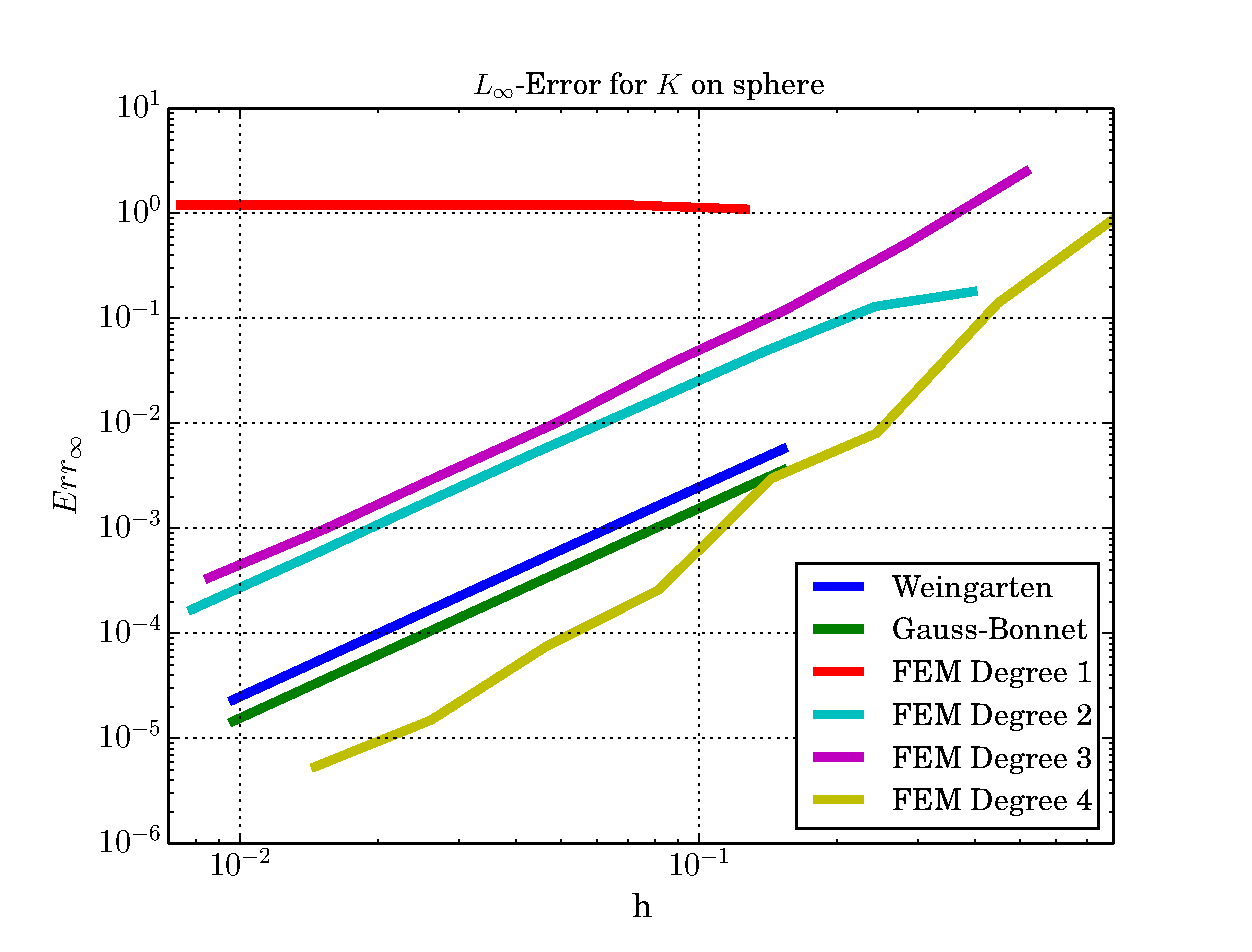
\includegraphics[width=\textwidth]{bilder/Curvature/sphere/ErrKLMax.eps}
    \end{minipage}\hfill
    \begin{minipage}[t]{0.49\textwidth}
       \centering\includegraphics[width=\textwidth]{bilder/Curvature/sphere/ErrHLMax.eps}
    \end{minipage}
    \caption[Fehlerplot (Krümmungen auf Sphäre)]
            {Log-Log-Plot der relativen diskreten \( L_{2} \)-Fehler (oben) und Maximumsfehler (unten) 
             für die Gaußsche Krümmung (links) und mittlere Krümmung (rechts) auf der Sphäre.}
    \label{figErrCompSphere}
    \centering\includegraphics[width=\textwidth]{bilder/Curvature/HeineB2k250kMeshGaussError.png}
    \caption[Gitterauflösung (quatrische Oberfläche)]
            {Das Gitter mit 1962 DOFs (\( h\approx0.34 \)) löst die beiden Wölbungen mit starker Krümmung
            nicht auf. Der Fehler (hier für \( K \) (Weingarten)) ist dort am größten. 
            Zum Vergleich ist ein Gitter mit 249642 DOFs (\( h\approx0.04 \)) halbtransparent
            dargestellt.}
    \label{figHeineBResolution}
  \end{figure}

  \begin{figure}
    \begin{minipage}[t]{0.49\textwidth}
       \centering\includegraphics[width=\textwidth]{bilder/Curvature/heineB/K250k.png}
    \end{minipage}\hfill
    \begin{minipage}[t]{0.49\textwidth}
       \centering\includegraphics[width=\textwidth]{bilder/Curvature/heineB/H250k.png}
    \end{minipage}\\
    \begin{minipage}[t]{0.49\textwidth}
       \centering\includegraphics[width=\textwidth]{bilder/Curvature/heineB/SK250k.png}
    \end{minipage}\hfill
    \begin{minipage}[t]{0.49\textwidth}
       \centering\includegraphics[width=\textwidth]{bilder/Curvature/heineB/SH250k.png}
    \end{minipage}\\
    \begin{minipage}[t]{0.49\textwidth}
       \centering\includegraphics[width=\textwidth]{bilder/Curvature/heineB/GB250k.png}
    \end{minipage}\hfill
    \begin{minipage}[t]{0.49\textwidth}
       \centering\includegraphics[width=\textwidth]{bilder/Curvature/heineB/LX250k.png}
    \end{minipage}
    \caption[Fehler (Krümmungen auf quatrischer Oberfläche)]
            {Absolute lokale Fehler für die Gaußsche Krümmung (links) und mittlere Krümmung (rechts) auf
            einer quatrischen Oberfläche
             ermittelt aus den Eigenwerten der diskreten Weingartenabbildung (mitte), dem
             Gauß-Bonnet-Operator (unten links) bzw. dem Krümmungsvektor (unten rechts).
             (249642 DOFs, \( h\approx0.04 \))}
    \label{figErrCurvHeineB}
  \end{figure}

  \begin{figure}
    \begin{minipage}[t]{0.49\textwidth}
       \centering\includegraphics[width=\textwidth]{bilder/Curvature/heineB/ErrKL2.eps}
    \end{minipage}\hfill
    \begin{minipage}[t]{0.49\textwidth}
       \centering\includegraphics[width=\textwidth]{bilder/Curvature/heineB/ErrHL2.eps}
    \end{minipage}\\
    \begin{minipage}[t]{0.49\textwidth}
       \centering\includegraphics[width=\textwidth]{bilder/Curvature/heineB/ErrKMax.eps}
    \end{minipage}\hfill
    \begin{minipage}[t]{0.49\textwidth}
       \centering\includegraphics[width=\textwidth]{bilder/Curvature/heineB/ErrHMax.eps}
    \end{minipage}
    \caption[Fehlerplot (Krümmungen auf quatrischer Oberfläche)]
            {Log-Log-Plot der relativen diskreten \( L_{2} \)-Fehler (oben) und Maximumsfehler (unten) 
             für die Gaußsche Krümmung (links) und mittlere Krümmung (rechts) auf einer quatrischen
             Oberfläche.}
    \label{figErrCompHeineB}
    \centering\includegraphics[width=\textwidth]{bilder/Curvature/LXDiameterTorus.png}
    \caption[Diameter u. Fehler f. Krümmungsvektor (Torus)]
            {Absolute lokale Fehler für die mittlere Krümmung berechnet aus dem Krümmungsvektor (links) und die Umkreisdurchmesser der
            Dreieckselemente (rechts).}
    \label{figLXDiameterTorus}
  \end{figure}

  \begin{figure}
    \begin{minipage}[t]{0.49\textwidth}
       \centering\includegraphics[width=\textwidth]{bilder/Curvature/heineC/K2k.png}
    \end{minipage}\hfill
    \begin{minipage}[t]{0.49\textwidth}
       \centering\includegraphics[width=\textwidth]{bilder/Curvature/heineC/H2k.png}
    \end{minipage}\\
    \begin{minipage}[t]{0.49\textwidth}
       \centering\includegraphics[width=\textwidth]{bilder/Curvature/heineC/SK2k.png}
    \end{minipage}\hfill
    \begin{minipage}[t]{0.49\textwidth}
       \centering\includegraphics[width=\textwidth]{bilder/Curvature/heineC/SH2k.png}
    \end{minipage}\\
    \begin{minipage}[t]{0.49\textwidth}
       \centering\includegraphics[width=\textwidth]{bilder/Curvature/heineC/GB2k.png}
    \end{minipage}\hfill
    \begin{minipage}[t]{0.49\textwidth}
       \centering\includegraphics[width=\textwidth]{bilder/Curvature/heineC/LX2k.png}
    \end{minipage}
    \caption[Fehler (Krümmungen auf Ellipsoid)]
            {Absolute lokale Fehler für die Gaußsche Krümmung (links) und mittlere Krümmung (rechts) auf
            einem Ellipsoid
             ermittelt aus den Eigenwerten der diskreten Weingartenabbildung (mitte), dem
             Gauß-Bonnet-Operator (unten links) bzw. dem Krümmungsvektor (unten rechts).
             (1962 DOFs, \( h\approx0.18 \))}
    \label{figErrCurvHeineC}
  \end{figure}

  \begin{figure}
    \begin{minipage}[t]{0.49\textwidth}
       \centering\includegraphics[width=\textwidth]{bilder/Curvature/heineC/ErrKL2.eps}
    \end{minipage}\hfill
    \begin{minipage}[t]{0.49\textwidth}
       \centering\includegraphics[width=\textwidth]{bilder/Curvature/heineC/ErrHL2.eps}
    \end{minipage}\\
    \begin{minipage}[t]{0.49\textwidth}
       \centering\includegraphics[width=\textwidth]{bilder/Curvature/heineC/ErrKMax.eps}
    \end{minipage}\hfill
    \begin{minipage}[t]{0.49\textwidth}
       \centering\includegraphics[width=\textwidth]{bilder/Curvature/heineC/ErrHMax.eps}
    \end{minipage}
    \caption[Fehlerplot (Krümmungen auf Ellipsoid)]
            {Log-Log-Plot der relativen diskreten \( L_{2} \)-Fehler (oben) und Maximumsfehler (unten) 
             für die Gaußsche Krümmung (links) und mittlere Krümmung (rechts) auf einem Ellipsoid.}
    \label{figErrCompHeineC}
  \end{figure}
%\section{Approximation der Krümmung}
%  \subsection{Beispiel: Krümmung Teil 1: Gauß-Bonnet-Operator}
%  \subsection{Beispiel: Krümmung Teil 2: Weingarten-Abbildung}
%  \subsection{Beispiel: Krümmung Teil 3: Krümmungsvektor}
%  \label{subsecKruemmungsvektor}

